
%%%%%%%%%%%%%%%%%%%%%%%%%%%%%%%%%%%%%%%%%%%%%%%%%%%%%%%%%%%%%%%%%%%%%%%%%%%%%%%%%%%%%%%%%%%%%%%%%%%%%%%%%%%%%%%%%%%%%%%%%%%%%%%%%%
\begin{criteria}{corr}\cite{EM99}\cite{DG10}
  An encoding is \emph{operational correspondent} if it is\footnote{This criteria is stronger than Gorla's criteria.}
	\begin{itemize}
		\item \mylabel{Complete}: $S\vred{\alpha}_1S'$ iff $\bkt{S}\vred{\phi(\alpha)}_2\asymp_2\bkt{S'}$;
		\item \mylabel{Sound}: if $\bkt{S}\vred{\alpha}_2T$, then there exists an $S'$ such that $S\vred{\gamma}_1S'$ and $T\vred{\beta}_2\asymp_2\bkt{S'}$, and $\alpha$, $\beta$ $\in$ $image(\phi)$.
  \end{itemize}
\end{criteria}

The index indicates relations in the source or target language.
I omit the use of indices if there is no confusion.

$\asymp$ is a equivalence relation, the function $\phi$ is the renaming policy that is defined along with the encoding.
The relation $\vred{}$ is the reflexive, transitive closure over $\ar{}$, the reduction relation. $\vred{\alpha}$ is $\vred{}$ itself, if $\alpha$ is a reduction label, or $\vred{} \ar{\alpha} \vred{}$ otherwise.
$\vred{\alpha}\cdots\vred{\beta}$ is defined in the obvious way.

The \myref{Comepelete} criteria forces the encoding to translate a transition in the source language into a transition in the target language, following or followed by a series of silent actions.

In \myref{Sound}, the values of $\alpha$, $\gamma$, $\beta$ follow one of the lines:

\begin{table}[h!]
  \begin{center}
    \label{tab:table1}
    \begin{tabular}{l|c|r} % <-- Alignments: 1st column left, 2nd middle and 3rd right, with vertical lines in between
      $\alpha$ & $\gamma$ & $\beta$ \\
      \hline
      $\in\Name_r$ & $\in\Name_r$ & $\in\Name_r$\\
      $\phi(\ell)$ & $\ell\notin\Name_r$ & $\in\Name_r$\\
      $\in\Name_r$ & $\ell\notin\Name_r$ & $\phi(\ell)$\\
    \end{tabular}
  \end{center}
\end{table}

The \myref{Sound} criteria forbids introducing irrelevant actions in the translation by restricting $\alpha, \beta$ in the image of the renaming policy.
It also serves as garbage collection, namely allows the encoded terms to reach intermediate states that do not directly originate from the source term.
%%%%%%%%%%%%%%%%%%%%%%%%%%%%%%%%%%%%%%%%%%%%%%%%%%%%%%%%%%%%%%%%%%%%%%%%%%%%%%%%%%%%%%%%%%%%%

\textbf{b)} There is no homomorphic, operational correspondent (Criterion \ref{crt:corr}) encoding from ABC to CCS, up to weak bisimulation.

Again consider the processes $P$ and $P|P$.

$\bkt{P|P} = \bkt{P}|\bkt{P}$ \footnotesize{(homomorphy)}\normalsize.

$P\vred{}x$ implies $\bkt{P}\vred{}S \wedge\, S\eqv \bkt{x}$ for some $S$ \footnotesize{(completeness)}\normalsize.
Suppose the path is
\[
	\pi_1 : \bkt{P}\ar{}\cdots\ar{} S
\]

$P\vred{}y$ implies $\bkt{P}\vred{}T$ where $T\eqv \bkt{y}$, with path
\[
	\pi_2 : \bkt{P}\ar{}\cdots \ar{} T
\]

We can compose $\pi_1$ and $\pi_2$ into
\[
	\pi_3 : \bkt{P|P} = \bkt{P}|\bkt{P}\ar{}\cdots\ar{} S|\bkt{P} \ar{}\cdots\ar{} S|T
\]

$(S \eqv \bkt{x}\wedge T \eqv \bkt{y})\implies S|T \eqv \bkt{x}| \bkt{y} = \bkt{x|y}$, since weak bisimulation is a congruence to parallel composition.

In conclusion, $\bkt{P|P}\vred{}\eqv\bkt{x|y}$, and this implies $P|P\vred{} Q\wedge \bkt Q \eqv \bkt{x|y}$ for some $Q$ \myref{sound}.

As shown in \fig{pgpp}, $Q$ can be either $P|P$ or $x|x$ or $y|y$.

If $Q=P|P$, $\bkt Q \eqv \bkt{x|y}$ implies $\bkt{P|P}\eqv \bkt{x|y}$



%%%%%%%%%%%%%%%%%%%%%%%%%%%%%%%%%%%%%%%%%%%%%%%%%%%%%%%%%%%%%%%%%%%%%%%%

\subsection{CCSS to \CSG}
\begin{proposition}{ccss-ccssg}
  There is a homomorphic encoding (w.r.t. all operators except prefixing) from CCSS to \CSG with two priorities.
\end{proposition}

\begin{proof}
  We first need to define in Table \ref{tab:accs} sets that represent all non-signal actions a CCSS process can potentially engage in.
  Let $e \in \Name_{CCS}$ a non-signal input action in CCSS, and $\bar{e} \in \overline{\Name_{CCS}}$ its corresponding output action.
  Set subtraction is defined in the usual way.
  \begin{table*}[t]
    \normalsize
    \centering
    \caption{Potential Non-Signal Action Sets for CCSS}
    \label{tab:accs}
    \framebox{
    $\begin{array}{lll}
    E(\tau.P) = \{ \epsilon \} &
    E(P + Q) = E(P) \cup E(Q) &
    E(A) = E(P)\ (A \defis P)
    \\[1ex]
    E(e.P) = \{ e_i \} &
    E(P | Q) = E(P) \cup E(Q) &
    E(P[f]) = \{ f(i) \mid i \in E(P) \}
    \\[1ex]
    E(\bar{e}.P) = \{ e_o \} &
    E(P\backslash L) = E(P) \backslash L &
    E(P\signals {s}) = E(P)
    \end{array}$}
  \end{table*}

  For readability, we write $\underline{\alpha}$ instead of $\alpha\hspace{-0.8mm}:\hspace{-0.8mm}0$ and $\alpha$ instead of $\alpha\hspace{-0.8mm}:\hspace{-0.8mm}1$.
  Let $\sum E(P) = \sum_{e\in E(P)}e$ and $\underline{E(P)} = \{\underline{e} \mid e \in E(P)\}$, the encoding is as follows:

  \begin{center}
  \hspace{-4.25cm}$\bkt{P\signals s} := X | \bkt{P},\ X \defis \ren{\overline{s}}.X + \sum \underline{E(P)} $\\[2ex]
  $\begin{array}{lll}
  \bkt{e.P} := \ren{e}.\overline{\underline{e_i}}.\bkt{P} &
  \bkt{\overline{e}.P} := \ren{\overline{e}}.\overline{\underline{e_o}}.\bkt{P} &
  \bkt{\tau.P} := \ren{\tau}.\overline{\underline{\epsilon}}.\bkt{P}
  \\[2ex]
  \bkt{P + Q} := \bkt{P} + \bkt{Q} &
  \bkt{P | Q} := \bkt{P} | \bkt{Q} &
  \bkt{A} := P'\ (A\defis P,\ P'=\bkt{P})
  \\[2ex]
  \bkt{P[f]} := \bkt{P}[f'] &
  \bkt{P\backslash L} := \bkt{P} \backslash \ren{L}
  \\[2ex]
  \end{array}$
  \end{center}

  The renaming policy $\ren{}$ satisfies $\ren{\overline{\alpha}} = \overline{\ren{\alpha}}$ and $\ren{e} = e\hspace{-0.8mm}:\hspace{-0.8mm}1 = e$, assuming that $\{a\hspace{-0.8mm}:\hspace{-0.8mm}1 \mid a \in \Name_{CCS} \}\subseteq \Name_{CCS^{sg}}$.
  $P[a\backslash b]$ means the process acquired by substituting every $a$ in $P$ with $b$.

  Again, the agent identifier $X$ is \emph{fresh}, in the sense that every encoding of a process including broadcast action prefix generates a different $X$.
  The relabelling function $f'$ satisfies $\ren{f(\alpha)}=f'(\ren{\alpha})$.
  $\ren{L}:=\{\ren{\alpha}\mid\alpha\in L\}$.

  \textbf{TO BE CONTINUED. }
\end{proof}
%%%%%%%%%%%%%%%%%%%%%%%%%%%%%%%%%%%%%%%%%%%



\begin{proof}
  By induction over the length of the computation $\C : \bkt{S} \vred{} \bkt{S'}$.
  The length of the computation is defined with the number of transitions in the computation, noted as $len(\C)$.

  Base case: if $len(\C) = 0$, we have that $\bkt S = \bkt{S'}$, thus $S = S'$, and the lemma is true.

  Step case: if $len(\C) = n > 0$, we prove that if the lemma is true for all $\C'$ where $len(\C') < n$, then the lemma is also true for $\C$.

  We prove the step case above with structural induction.

  From the encoding we can see, all high prioritised actions have a low prioritised action as prefix, which means that the first transition in $\C$ cannot be labelled with high priority.
  At the same time, \lem{pree} tells us that the first transition cannot be labelled with medium priority.
  Thus the first transition must be a $\tau_l$-labelled transition.

  Suppose the step case is true for some $P, Q, P_i \in \St_{ABC}$ ($i\in I$, $I$ an index set).

  Trivially, the step case is true for $S=\nil$, since there is no outgoing transition from $S$ and thus the length of any computation $\C$ of $S$ satisfies $len(\C) = 0$, the condition in the step case does not hold and the implication is always true.
  \begin{itemize}
    \item \emph{Prefixing:}
    If $S=\alpha.P$, then $S\ar{\alpha}P$.
    The encoding of $S$ depends on $\alpha$.
    \begin{itemize}
      \item If $\alpha\in\HS_{ABC}$, then $\bkt{S} = \alpha_l.\bkt{P}$, and there is no outgoing computation from $\bkt S$ with length greater than $0$.
      The same if $\alpha\in\B?$.
      \item If $\alpha = \tau$, then $\bkt{S} = \tau_l.\bkt{P}$, which means that $\bkt S \ar{\tau_l} \bkt P$ is the only outgoing transition from $\bkt{S}$.
      This means that any computation $\C : \bkt S \vred{} \bkt S'$ must be in the form: $\bkt S \ar{\tau_l} \bkt{P}\vred{}\bkt{S'}$.

      If $len(\C) = 1$, then $\bkt S \ar{\tau_l} \bkt{P}$ and $S\ar{\tau}P$, the step case is true.

      If $len(\C) > 1$, then $len(\C) = 1 + len(\C')$, where $\C' : \bkt{P}\vred{}\bkt{S'}$ and $len(\C') > 0$.


    \end{itemize}

    Since the computation $\C': \bkt{P}\vred{}\bkt{S'}$ has length less than $len(\C)$, we can use the induction hypothesis on $P$ and conclude with $P\vred{}S'$.
    Because $S\ar{}P$ and $P\vred{}S'$, we have that $S\ar{}S'$ for any computation $\C$.

    If $\alpha \in \B!$, then $\alpha = b!$ for some $b\in \B$.
    $\bkt{S} = \tau_l.(\overline{b_h}.X + \tau_m.\bkt{P})$ where $X\defis\overline{b_h}.X + \tau_m.\bkt{P}$.
    We can see that the only computation is $\bkt S \ar{\tau_l} t \ar{\tau_m} \bkt P$ where $t=\overline{b_h}.X + \tau_m.\bkt{P}$.
    Because $t\ar{\tau_m}$, we know from \lem{pree} that $t$ is not an encoding of any ABC process.
    Thus any computation $\C : \bkt S \vred{} \bkt{S'}$ must be in the form: $\bkt S \ar{\tau_l} t \ar{\tau_m} \bkt P \vred{} \bkt{S'}$.
    Again we use the induction hypothesis on $P$ and prove the step case.

    \item \emph{Choice:} Suppose $S=\sum_{i\in I}P_i$

		\item \emph{Parallel composition:} Suppose $S = P | Q$, $S \ar{b!} S'$, then $\bkt{S} = \bkt{P}| \bkt{Q}$.

    \item \emph{Agent Identifier:} Suppose $S\defis P$, the proof is again similar to that in Lemma \ref{lem:hc-comp}.

    \item \emph{Relabelling:} Suppose $S = P[f]$, then $\bkt{S} = \bkt{P}[f']$ where $\ren{f(\alpha)}=f'(\ren{\alpha})$ and $f'(\alpha) = \alpha$ if $\alpha \notin image(\varphi_{\bkt{}})$.

    \item \emph{Restriction:} Suppose $S=P\backslash L$, then $\bkt{S} = \bkt{P}\backslash \ren{L}$.


  \end{itemize}









    \begin{itemize}
      \item Suppose $\bkt S \ar{\tau_l} \bkt{S'}$, then it must originate from a handshake communication or a $\tau$-labelled transition in the source language.
      Otherwise suppose this transition originated from a broadcast action in the source language, then the target state of this transition must have an outgoing transition labelled with $\tau_m$ (please refer to the encoding), which according to \lem{pree}, is not an encoding of any ABC process, and this contradicts with the fact that the target state of this transition is the encoding of process $S'$.

      If the transition $\bkt S \ar{\tau_l} \bkt{S'}$ originated from a $\tau$-labelled transition
    \end{itemize}
  \end{proof}





  if a process $S\in\St_{CCS^{sg}}$ is an encoding of some term in $\St_{ABC}$, then it
  \begin{enumerate}[(1)]
    \item \label{itm:1} has as prefix low-prioritised actions or high-prioritised input/output actions;
    \item \label{itm:2} contains high-prioritised output actions, only if it has a $\tau_l$ as prefix;
    \item \label{itm:3} contains $\tau_m$, only if this $\tau_m$ has a $\tau_l$ or $b_h$ for some $b$ as prefix;
    \item \label{itm:4} has no handshake action with medium priority;
    \item \label{itm:5} after a high-prioritised input action, always transform into a process that can perform $\tau_m$ ;
    \item \label{itm:6} does not include $\tau_h$ as a subterm;
    \item \label{itm:7} contains $c_l$ for $c\in\HS_{ABC}$ only if it is part of an encoding of a handshake action in ABC, and $c_l$ is followed by the encoding of some ABC term.
  \end{enumerate}

  The effect of renaming does not invalidate the above statements, because it only maps silent action to silent action, and it does not change priority level (please refer to Section \ref{sec:ccssg}).











      If $s_n$ is a state on some computation
      \[
      \pi : \bkt{S} \ar{} s_1 \ar{} s_2 \ar{} \cdots \ar{} s_n
      \]
      such that $\forall i < n,\ \nexists S''\in\St_{ABC}:\ s_i = \bkt{S''}$ and $\exists S\in\St_{ABC} \wedge s_n = \bkt{S'}$.
      In other words, $\bkt{S}\vred{}\bkt{S'}$ with $\bkt{S'}=s_n$.

  \begin{shaded}
    From here to the end of this lemma (Lemma 13) is not fixed.

    %TODO: stopped here.

    Lemma 14 is fixed.
  \end{shaded}

  The execution of $\tau_l$ exposes a $Y$ as subterm of $p_1$ where $Y\defis \overline{e_h}.Y + \tau_m.\bkt{P'}$ for some $P'$, and $P\ar{e!}P'$, as we can see from the encoding.
  This means, $p_1$ is able to do $\tau_m$ and reach state $\bkt{P'}$, or $\overline{e_h}$ and return to $p_1$, which implies that $p_1$ does not do any action with low priority, for it would be preempted by the outgoing $\tau_m$ from $p_1$.
  It also does not do any other $\tau_m$, because all other $\tau_m$ have prefixes and $p_1$ must execute the prefixing actions before executing any other $\tau_m$ \ref{itm:3}, and there is no handshake action with medium priority as subterm in either $\bkt{P}$ or $p_1$ \ref{itm:3}.
  However, $p_1$ can possibly do some other actions with high priority that we do not explicitly know.

  The process graph of $p_1$ is shown in Figure \ref{fig:pgp1q2}, dotted arrow means actions that the processes can possibly do that we have no knowledge of; crossed arrow means actions that the processes cannot do.

  \begin{figure}
    \centering
    \caption{Process Graph of $p_1$ and $q_2$}
    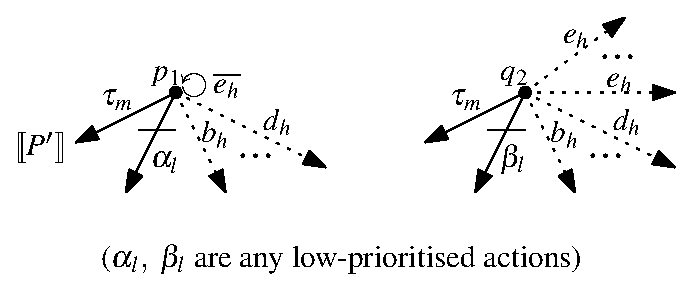
\includegraphics[width = 0.5\textwidth]{images/pgp1q2.eps}
    \label{fig:pgp1q2}
  \end{figure}

  Since $s_1 = p_1|q_1$ and $p_1\ar{\tau_m}\bkt{P'}$, $s_1$ cannot do any low-prioritised actions, which implies that $s_1\ar{}s_2$ is either labelled with $\tau_m$ or $\tau_h$.
  If $s_1\ar{\tau_m}s_2$, then it decomposes into $p_1\ar{\tau_m}\bkt{P'}$ for some $P'$, $q_1\ar{\nil}q_2 \wedge q_1 = q_2 = \bkt{Q}$, because there is no outgoing transition from $q_1$ labelled with $\tau_m$ \ref{itm:3}\ref{itm:4}.
  The computation $\pi$ then becomes
  \[
    \bkt{S} \ar{\tau_l} s_1 \ar{\tau_m} s_2 = \bkt{P'}|\bkt{Q}
  \]
  $s_n = s_2$, $S\ar{e!}S' = P'|Q$.

  If otherwise $s_1\ar{\tau_h}s_2$, then it must decompose into
  \[p_1\ar{\overline{e_h}}p_2;\ q_1\ar{e_h}q_2\ \ref{itm:2}\]
  and the execution of $e_h$ exposes $\tau_m$ \ref{itm:5}.
  The process graph of $p_2$ is in Figure \ref{fig:pgp1q2}.

  As shown by the process graph of $p_1$ in \fig{pgp1q2}, $p_1$ does an $\overline{e_h}$ and return to a state that is identical with itself, thus $p_2=p_1$.
  Also, there is no outgoing transition from $p_1$ or $p_2$ labelled with an output action that is not $\overline{e_h}$.

  As a result, the computation starting from the parallel composition $p_2 | q_2$ must consist only transitions labelled with $\tau_h$, which all originated from the handshake communication of $\overline{e_h}$ and $e_h$, until there is no more $\tau_h$ possible, i.e. all $\overline{e_h}$ in the process graph of $q_2$ are consumed.

  The reason behind is that $\tau_h$ preempts all transitions with lower priority, thus no successor of $q_2$ can do a $\tau_l$ and expose any output action labelled with high-prioritised action \ref{itm:2}; at the same time, after executing $\overline{e_h}$, $p_2$ ($p_1$) always returns to itself, where no outgoing output high-prioritised action other than $\overline{e_h}$ is possible.

  We note the state as $q_i$ by which there is no more exposed $e_h$.
  The (partial) decomposition of $\pi$ is:
  \begin{align*}
    & \pi_1 : \bkt{P} \ar{\tau_l} p_1 \ar{\overline{e_h}} p_2 \ar{\overline{e_h}} \cdots \ar{\overline{e_h}} p_i = p_1 ;\\
    & \pi_2 : \bkt{Q} \ar{\nil} q_1 \ar{e_h} q_2 \ar{e_h} \cdots \ar{e_h} q_i .
  \end{align*}
  and all the intermediate states are not a translation of any ABC terms, because they can all do $\tau_m$ actions \ref{itm:3}.

  The decomposition continues before reaching states such that $s_n = p_n|q_n$ and $s_n$ is an encoding of some ABC term, which means $p_n$, $q_n$ must also be encodings of some ABC terms (the proof is not complicated and we leave it out).

  To reach states $p_n$ and $q_n$, $p_i$ (at some point) must do a $\tau_m$ action and reach the state $\bkt{P'}$ in \fig{pgp1q2}, where $P\ar{e!}P'$ according the encoding; $q_i$ must execute all its exposed $\tau_m$ \ref{itm:3}. %, consuming all unprotected sequences of $e_h.\tau_m$ in $\bkt{Q}$, leaving $\bkt{Q_2},\ \bkt{Q_3},\ \dots,\ \bkt{Q_i}$ connected with \CSG operators except for action prefixing, where $e?.Q_j$ are subterms in $Q$, for all $2\leq j$.

  The decomposition of $\pi$ continues, for instance:
  \begin{align*}
    & \pi_1' : p_i \ar{\tau_m} p_{i+1} \ar{\nil} \cdots \ar{\nil} p_{2i};\\
    & \pi_2' : q_i \ar{\nil} q_{i+1} \ar{\tau_m} \cdots \ar{\tau_m} q_{2i}.
  \end{align*}
  and $q_{2i}$ is the encoding of $Q'$ for some $Q'$, and $Q\ar{e?}Q'$
  Also, $p_{2i} = \bkt{P'}$ and $P\ar{e!}P'$.
  At the same time, all $q_k$ where $i < k < 2i$ are not encodings of any ABC terms because of the outgoing $\tau_m$ transitions \ref{itm:3}.
  Thus $s_n = p_{2i}|q_{2i}$ is the first state such that it is an encoding of some ABC term.

  If we postpone the execution of $p_i \ar{\tau_m} p_{i+1}$, all possible decompositions are represented.

  In conclusion, any computation $\pi$ that starts with $\bkt{S}\ar{\tau_l}s_1\ar{\tau_h}$ can be decomposed into $\pi_1\pi_1'$ and $\pi_2\pi_2'$ such that $S\ar{e!}S'$ with $S = P|Q$, $P\ar{e!}P'$, $Q\ar{e?}Q'$, $S' = P'|Q'$.


  In homomorphic encodings, choice operator is encoded into choice operator: $\bkt{\nil\signals{s} + y} = \bkt{\nil\signals{s}} + \bkt y$.
